\section{N-grams language models}\label{sec:n-grams}

An n-gram is a contiguous sequence of items (typically letters or words) that are extracted from an information source (normally text, speech, images or \gls{dna}). By counting the n-grams in a knowledge corpus they can be used to create probabilistic language models for predicting the next item given a context. This is useful when developing speech recognizers and \gls{ocr} systems because the n-gram language model can help disambiguate items in the recognition process. Moreover they can be used for implementing text generators or suggestion / auto-complete systems and can also be applied to improve the efficiency of compression / search algorithms.



\subsection{Rank-frequency graphs}

Rank-frequency graphs are useful to analyze the word / n-gram diversity of a given text corpus. They are usually plotted in logarithmic scale and have the word rank in the X axis and the word frequency in the Y axis. They are also useful to check if a given text corpus follows the Zipf's law \cite{Piantadosi2014}, which states that the frequency of a given word in a text corpus is inversely proportional to its rank in the frequency table (as shown in \cref{eq:zipf-law}).

\begin{equation}\label{eq:zipf-law}
f(r) \propto \frac{1}{r^\alpha}
\end{equation}

Analyzing \crefrange{fig:rank-frequency-unigram}{fig:rank-frequency-pentagram} it can be seen that the dataset unigrams to pentagrams follow roughly the Zipf's law. Moreover, the alpha value introduced in \cref{eq:zipf-law} that best fits the plotted data starts at 0.25 in the first section, then increases to 0.5 in the middle section and becomes 1.0 in the last section. This is a typical behavior found in most languages \cite{NemethZainko2003}.

\begin{figure}[hb]
	\centering
	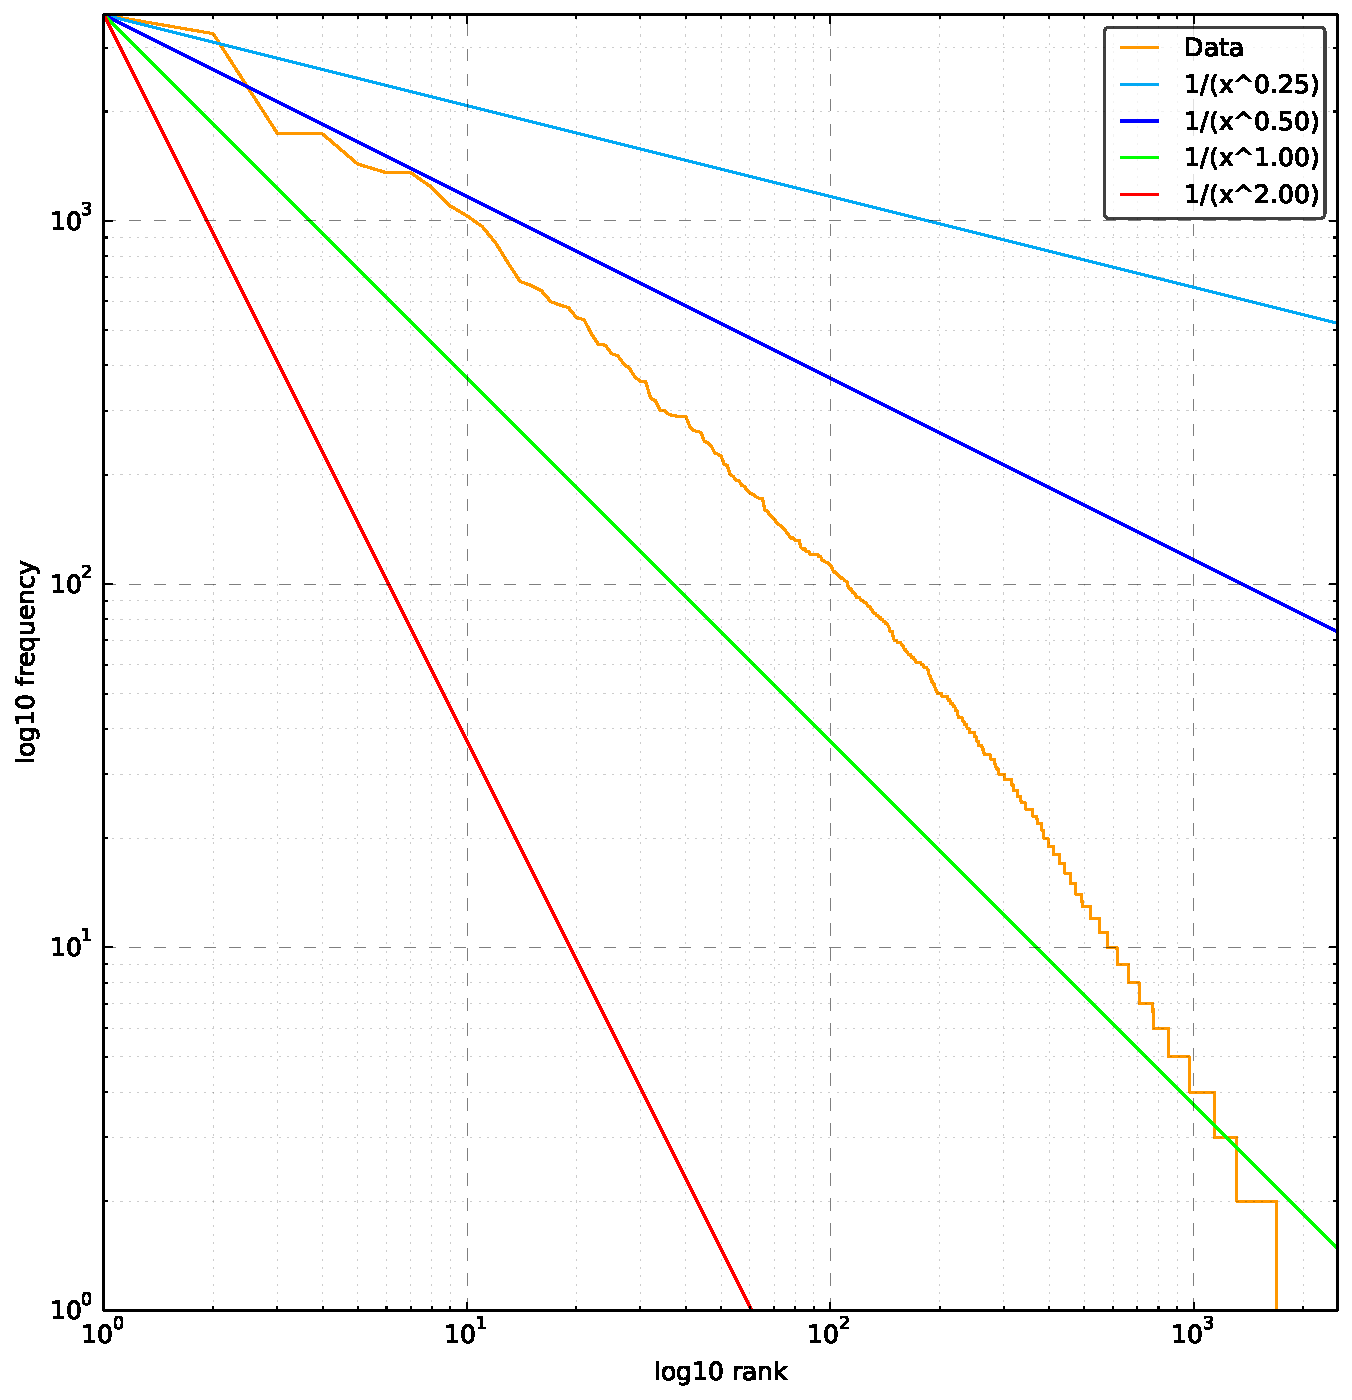
\includegraphics[width=0.9\linewidth]{figures/frequency-graphs/1-gram}
	\caption{Unigram rank-frequency graph of tokenized dataset}
	\label{fig:rank-frequency-unigram}
\end{figure}

\begin{figure}[ht]
	\centering
	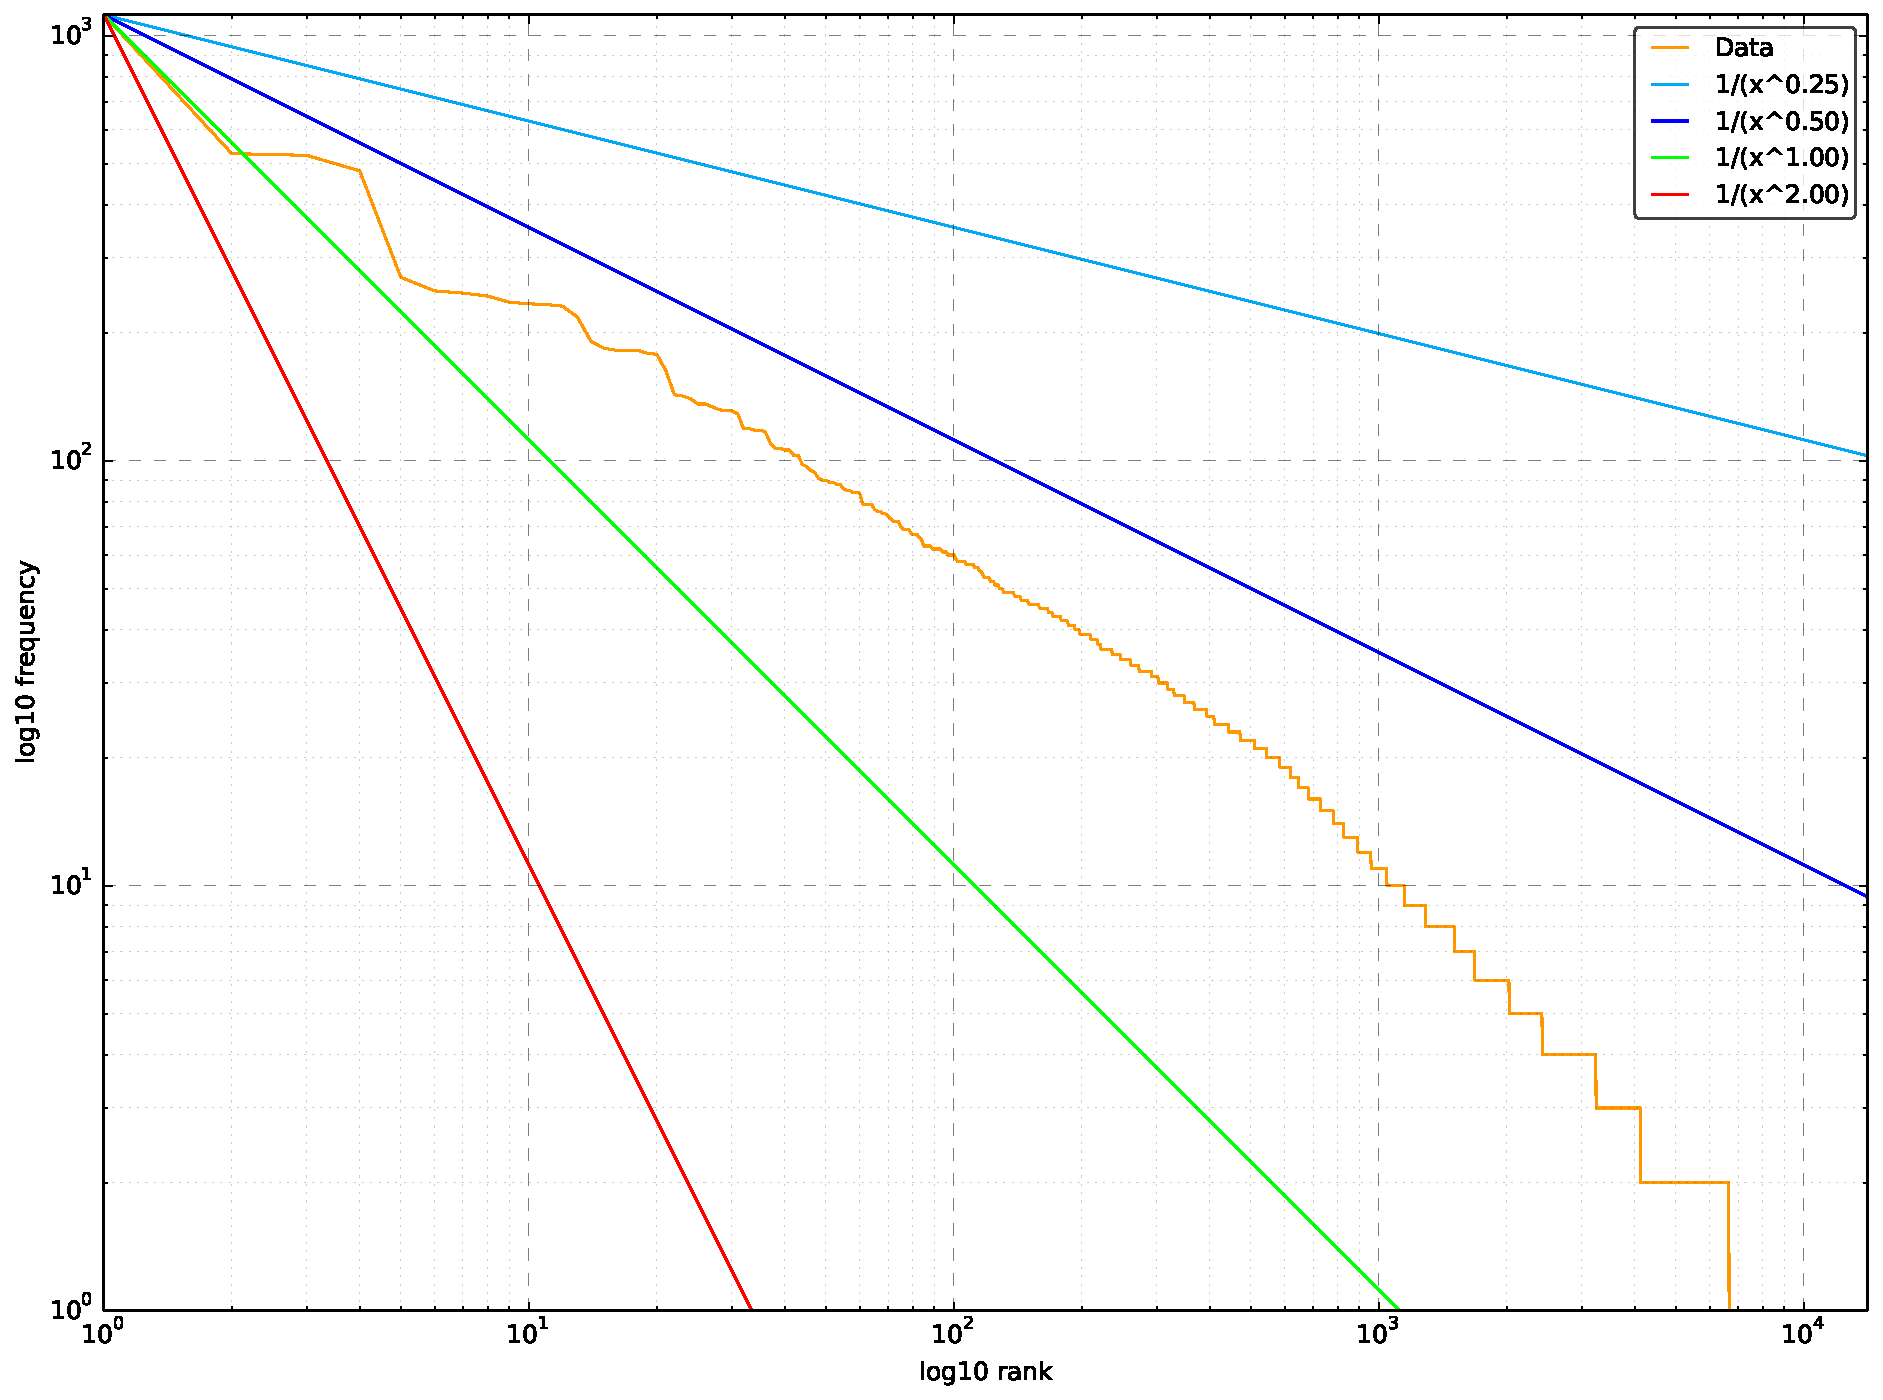
\includegraphics[width=0.9\linewidth]{figures/frequency-graphs/2-gram}
	\caption{Bigram rank-frequency graph of tokenized dataset}
	\label{fig:rank-frequency-bigram}
\end{figure}

\begin{figure}[ht]
	\centering
	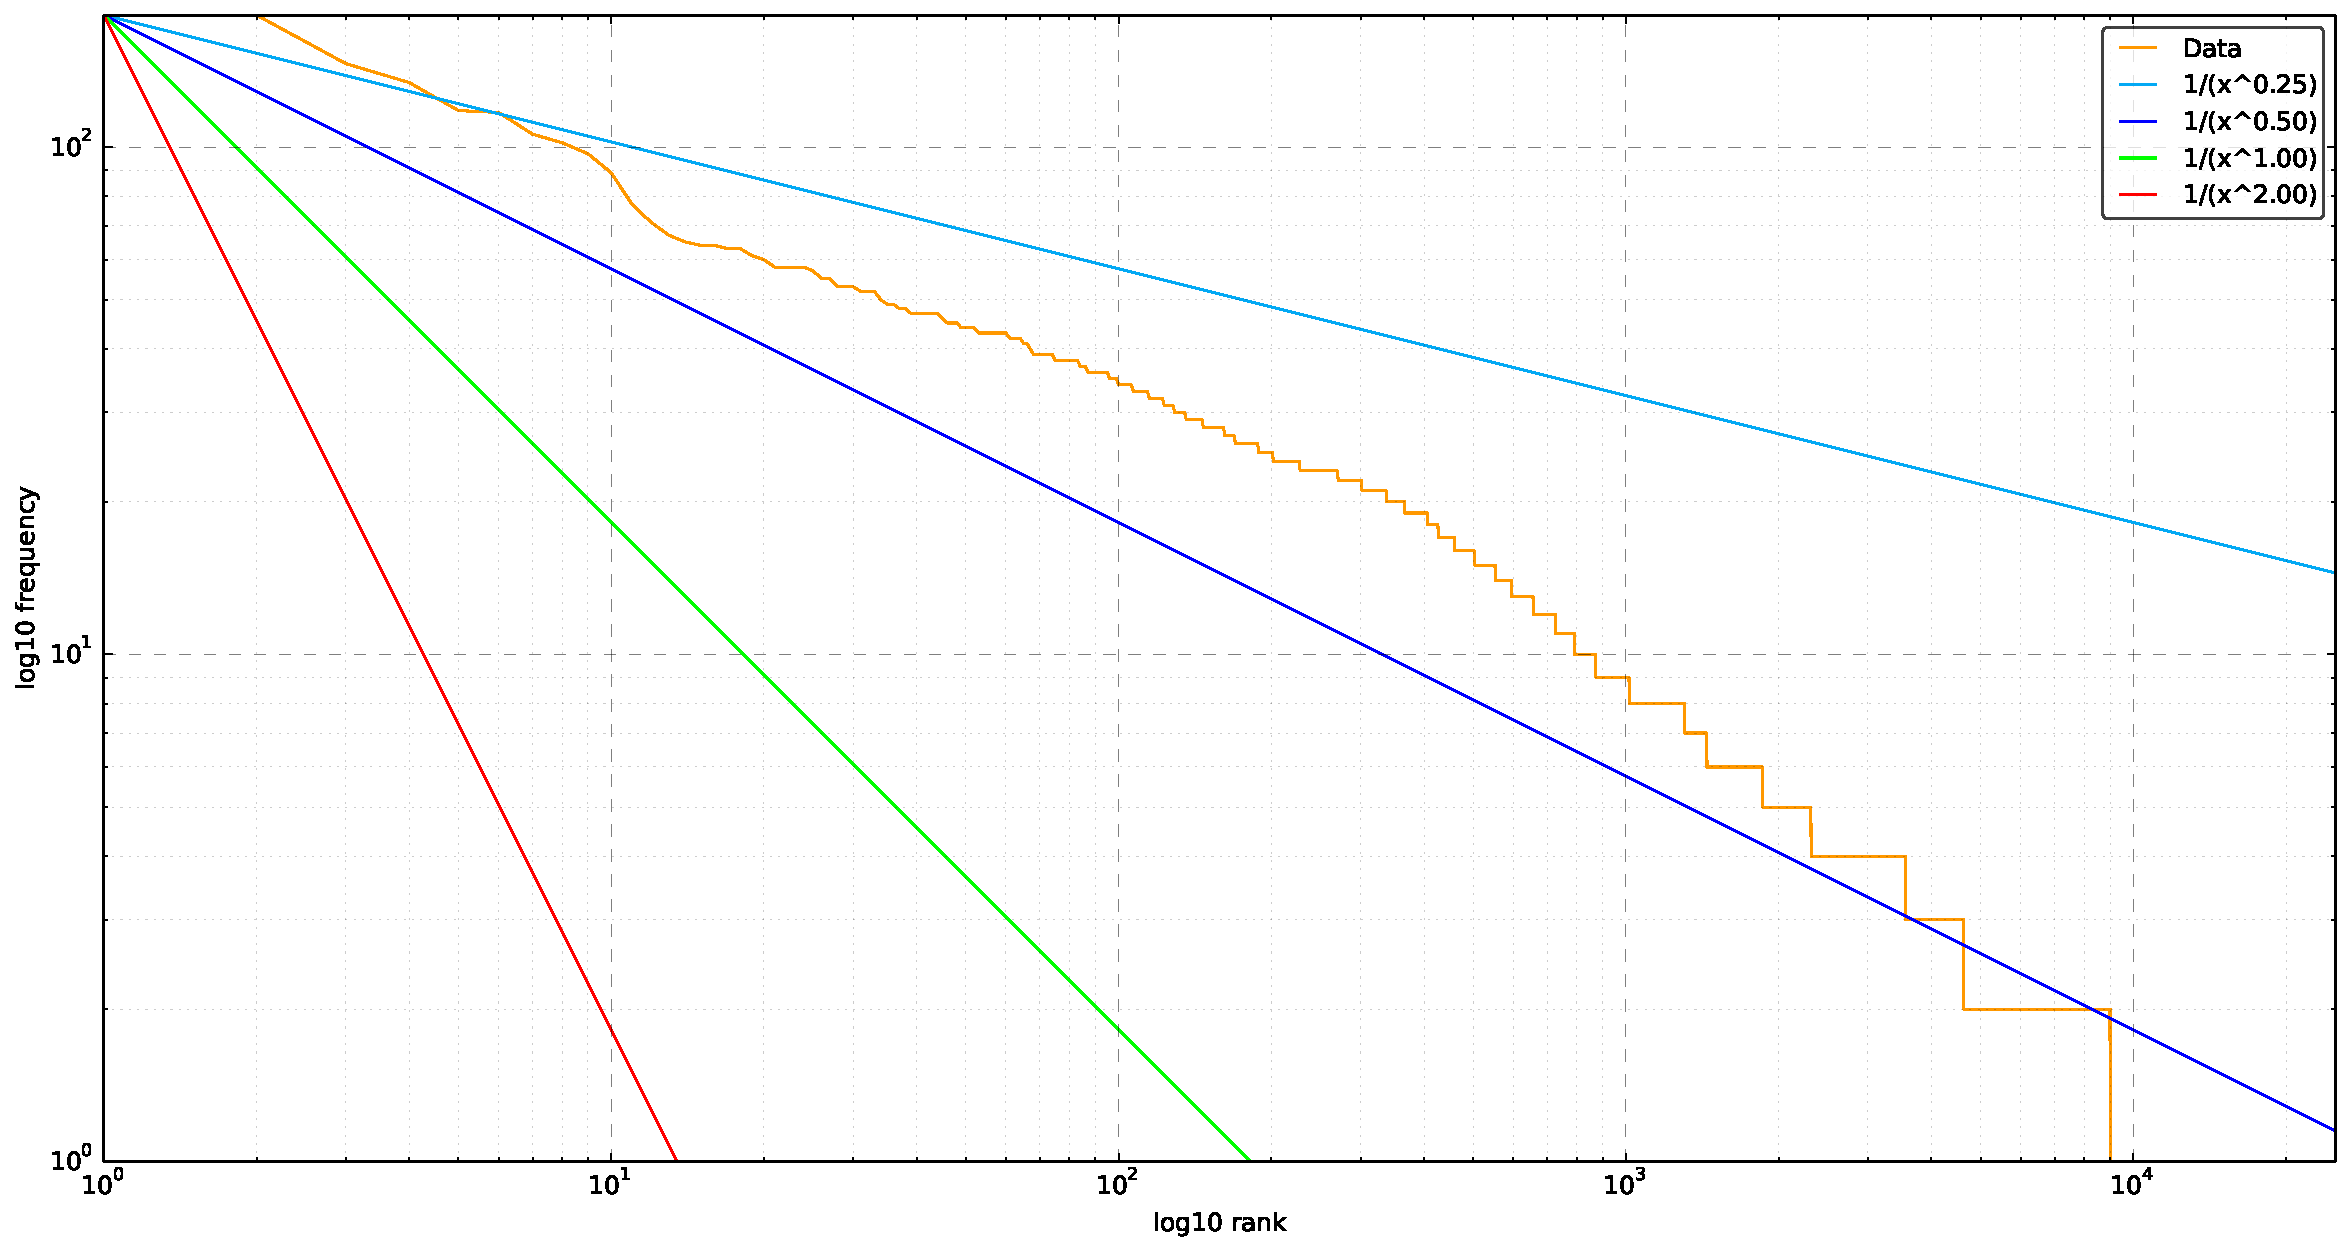
\includegraphics[width=0.9\linewidth]{figures/frequency-graphs/3-gram}
	\caption{Trigram rank-frequency graph of tokenized dataset}
	\label{fig:rank-frequency-trigram}
\end{figure}

\begin{figure}[ht]
	\centering
	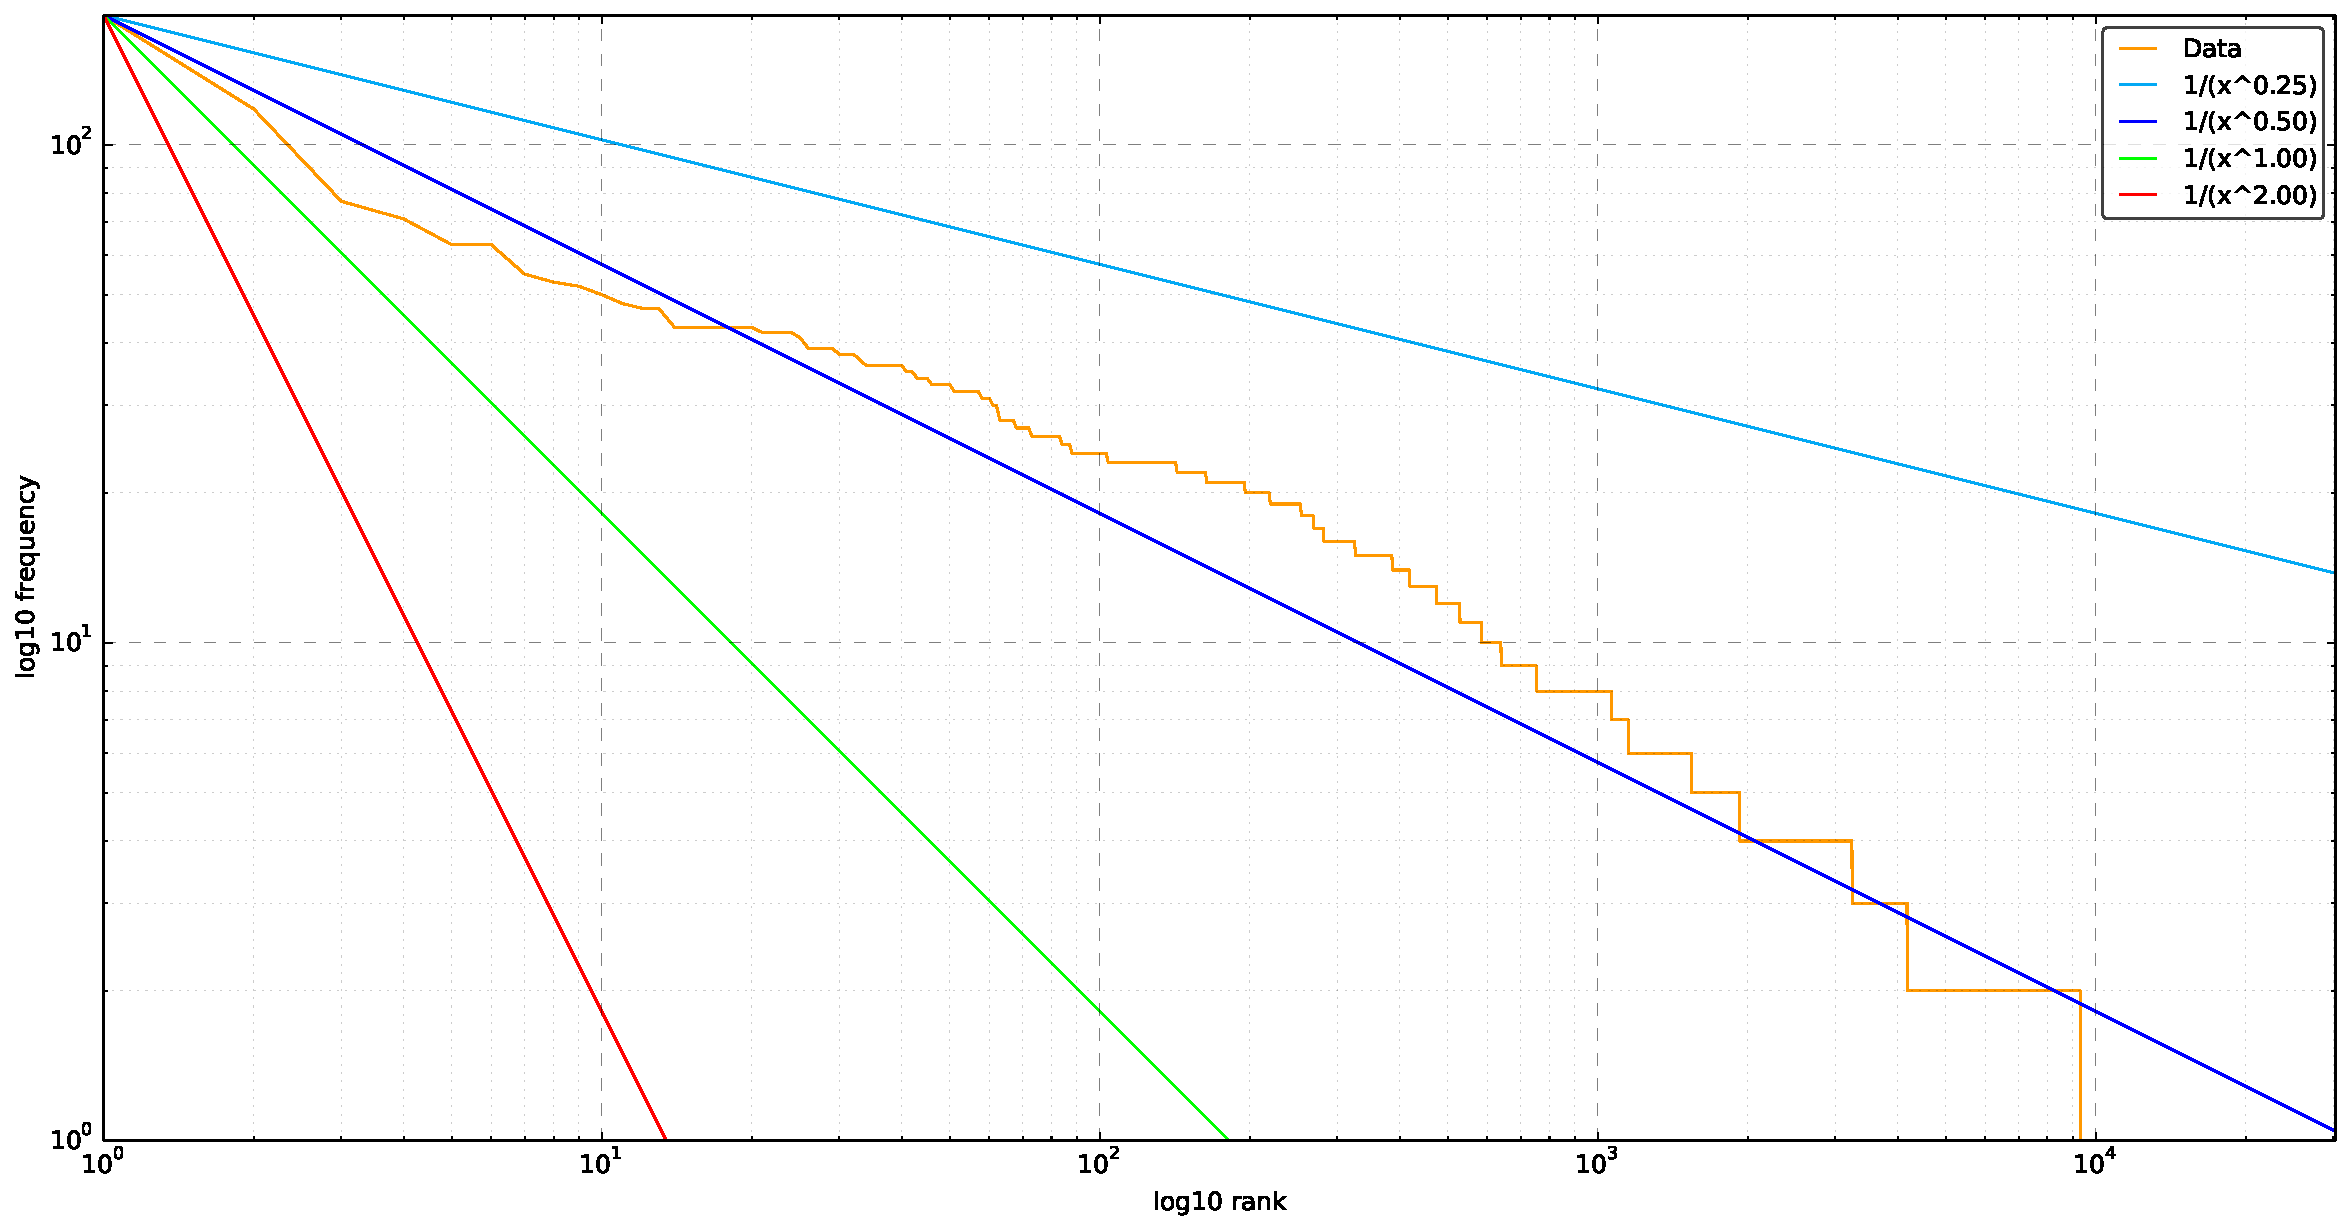
\includegraphics[width=0.9\linewidth]{figures/frequency-graphs/4-gram}
	\caption{Tetragram rank-frequency graph of tokenized dataset}
	\label{fig:rank-frequency-tetragram}
\end{figure}

\begin{figure}[ht]
	\centering
	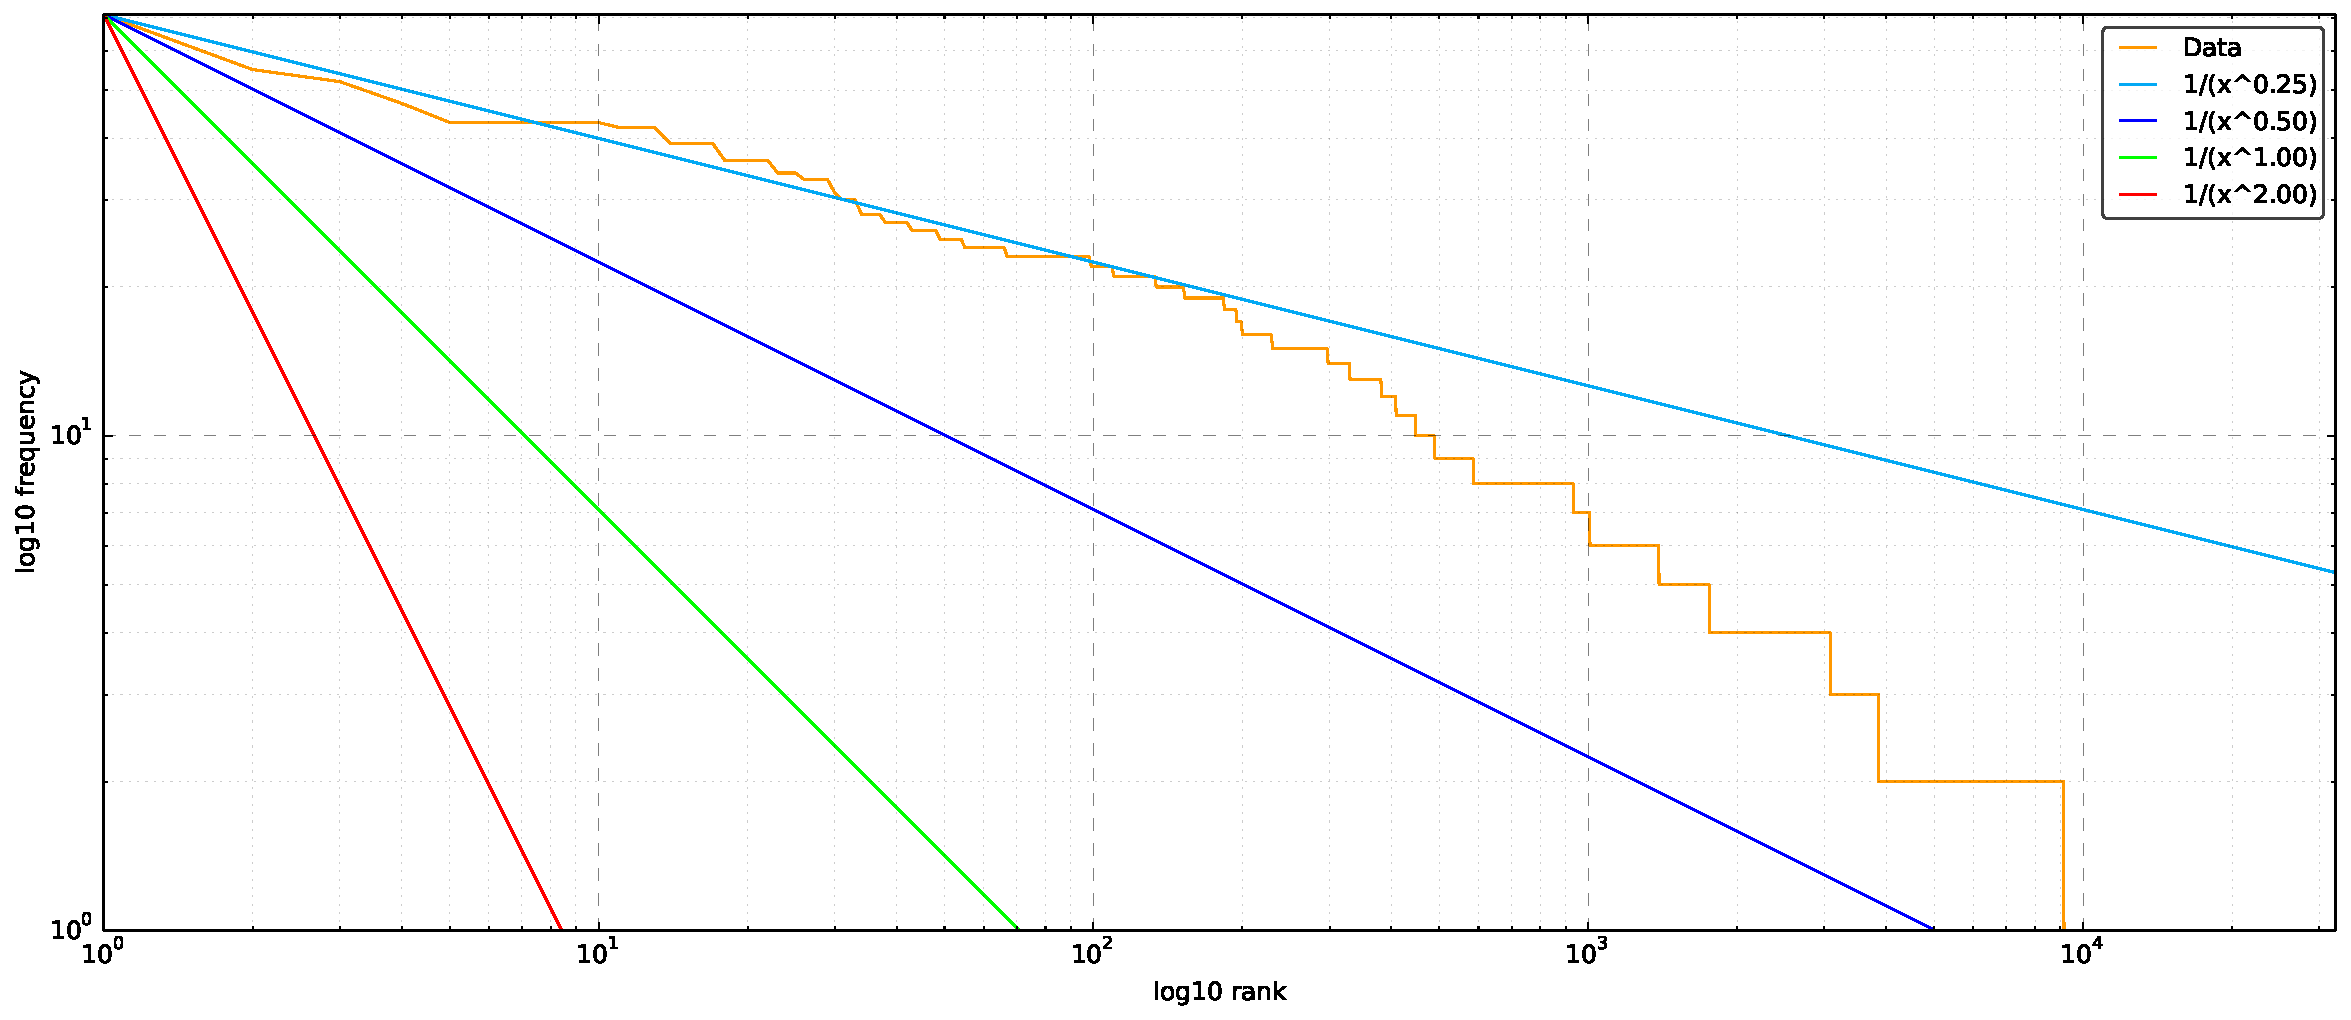
\includegraphics[width=0.9\linewidth]{figures/frequency-graphs/5-gram}
	\caption{Pentagram rank-frequency graph of tokenized dataset}
	\label{fig:rank-frequency-pentagram}
\end{figure}



\subsection{Most common and uncommon n-grams}

FF.



\subsection{N-grams interpolation}

FF.



\subsection{N-grams models smoothing}

FF.



\subsection{Sentence generation using n-gram models}

FF.



\subsection{N-gram models perplexity}

FF.
